\documentclass{article}
\usepackage{CJKutf8}
\usepackage{multirow}
\usepackage{listings}
\usepackage{graphicx}
\usepackage{subfigure}
\usepackage[colorlinks,linkcolor=red]{hyperref}
\begin{CJK}{UTF8}{gbsn}
\usepackage[framed,numbered,autolinebreaks]{mcode}
\begin{document}
\title{通信系统第三次作业}
\author{王亭午, 无210班, 2012011018}
\date{2015年5月30号}
\maketitle
\section{作业一}
多径信道和时域判决反馈均衡器的仿真练习。随机产生长为10000bit的01序列,采用
QPSK调制,格雷码映射。信道模型为(1)直射信道 h=1; (2)多径信道,强度 h\_dB \(=[0,-6,-8,-10]\)(单位为 dB);
对应的时延 h\_time \(=[0,2,5,16]\)(单位为符号周期);
假设接收机处的信噪比SNR=15dB。\\
本题所有代码及版本历史都在我的github上留有副本。
如果习惯在github上阅读代码可以在线浏览。我的github \url{https://github.com/WilsonWangTHU/commSystem}。
\begin{figure}[b!]
\centering
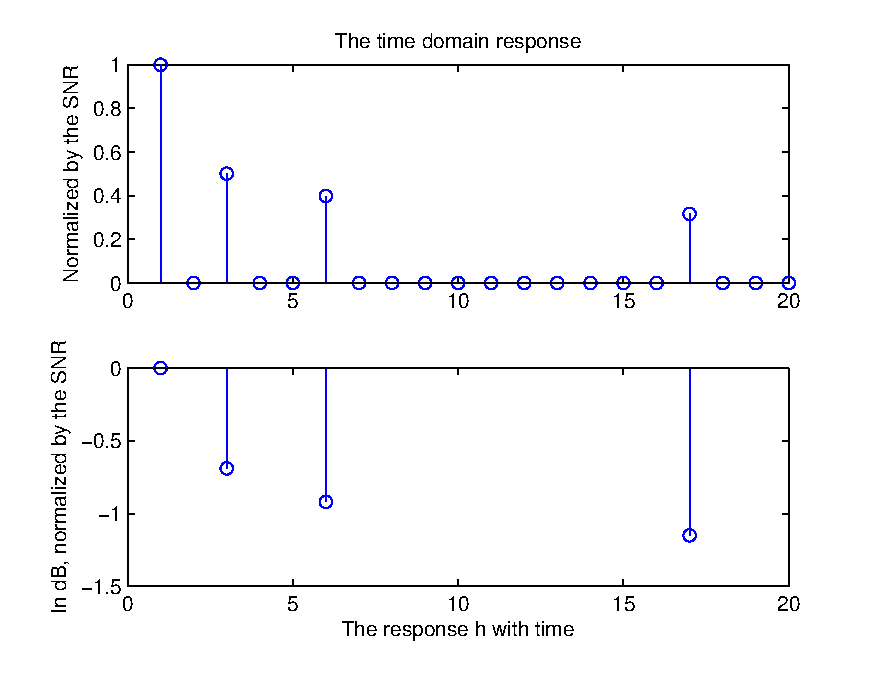
\includegraphics[width=9cm]{1.eps}
\caption{}
\end{figure}
\subsection*{a. 时域冲激响应}给出信道(2)的时域冲激响应图\\
代码在main.m中,逻辑比较简单,不在这里列出来。效果图Fig. 1,Fig. 1下半图为对数坐标小的图。
\subsection*{b. 星座图}分别给出序列经过信道前后的星座图\\
可以看到,在通过我们的信道之后,星座图出现了非常大的变化。原图中的信号全部集中在4个qpsk传输点上。
而在接收端,大量的接受的qpsk信号都偏离了原来的位置,信号之间互相干扰。
值得注意的是,接受信号存在明显的模式(pattern),这为之后的滤波提供了可能。
\begin{figure}[h]
\begin{minipage}[t]{0.5\linewidth}
\centering
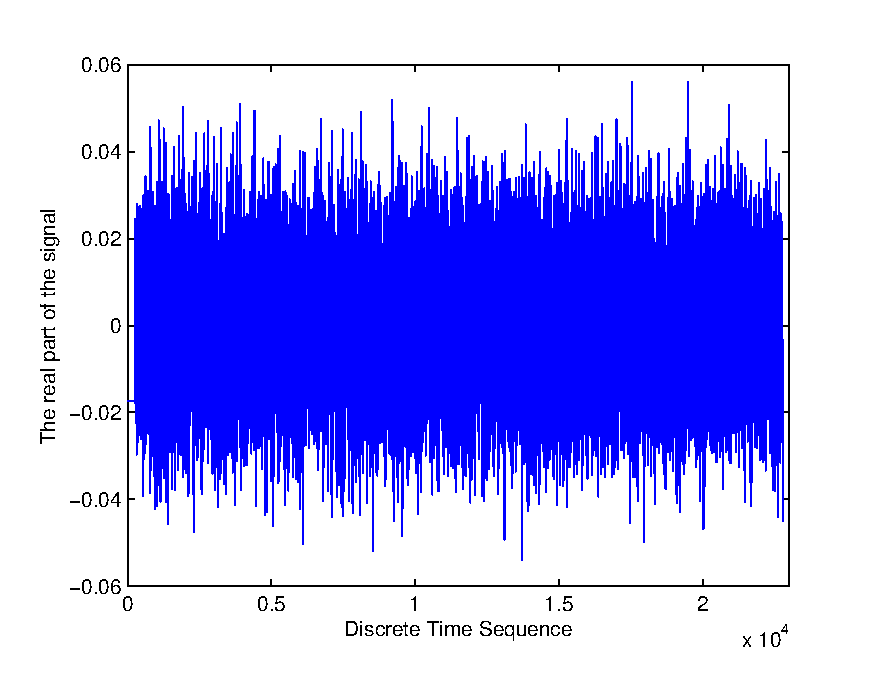
\includegraphics[width=2.2in]{2.eps}
\caption{输入前星座图}
\label{fig:side:a}
\end{minipage}%
\begin{minipage}[t]{0.5\linewidth}
\centering
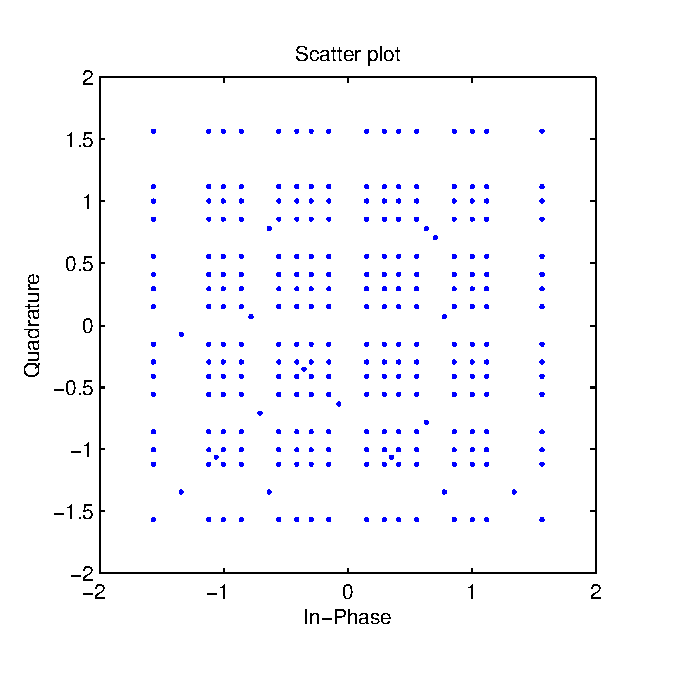
\includegraphics[width=2.2in]{3.eps}
\caption{输入后星座图}
\label{fig:side:b}
\end{minipage}
\end{figure}
\subsection*{c. LMS}假设已知该序列的前500个点,作为训练序列。采用时域的判决反
馈均衡器进行均衡,采用LMS准则,均衡器的抽头数量为32。给出训练过程中的误差曲线和未知序列经过均衡处理后的星座图。\\
代码为main2.m,迭代参数的代码如下:
值得注意的是,迭代的初始点非常的重要。在实际情况中,我们选取\(W_1\)最大,
因为我们知道直射信道依然是最好的信道。如果初始点选择错误,很有可能会发生发散性震荡。
在迭代中,我使用了归一化LMS算法,\(c_0 = 0.01,\,\mu = 0.001\)。
\begin{equation}
\mu' = \frac{\mu}{c_0 + \frac{1}{L}\sum\nolimits|x_k|^2}
\end{equation}
\begin{lstlisting}
function weight = LMS(raw_output, true_output, nWeight)
% raw_output -> x, true_output -> y, y_i = \sum(xTw)

% initialize the weight factor
weight = zeros(nWeight, 1);
weight(nWeight) = 1;

mu = 0.001;
c0 = 0.01;
mu_unified = mu / (c0 + sum(raw_output' * raw_output) ...
    / nWeight);
% append nWeight zeros to enable the calculations
raw_output = [zeros(nWeight - 1, 1); raw_output];
% loop until convergence
lastTimeError = 0;
while 1
    % renew the raw output
    predict_output = zeros(length(true_output), 1);
    for iWeight = 1: 1: nWeight
        predict_output = predict_output + weight(iWeight) * raw_output(iWeight: length(true_output) + iWeight - 1);
    end
    
    % get the error of the target function
    target_error = true_output - predict_output;
    
    % break if stoped
    if abs(sum(target_error' * target_error) - lastTimeError) < 0.01
        break
    end
    
    lastTimeError = sum(target_error' * target_error);
    %fprintf('The overall error is now %f\n', lastTimeError);
    
    for iWeight = 1: 1: nWeight
        % get the unifying descedent steps and decent
        descent = target_error' * raw_output(iWeight: length(true_output) + iWeight - 1);
        weight(iWeight) = weight(iWeight) + 2 * mu_unified * descent;
    end
end
\end{lstlisting}
\begin{figure}[h]
\begin{minipage}[t]{0.5\linewidth}
\centering
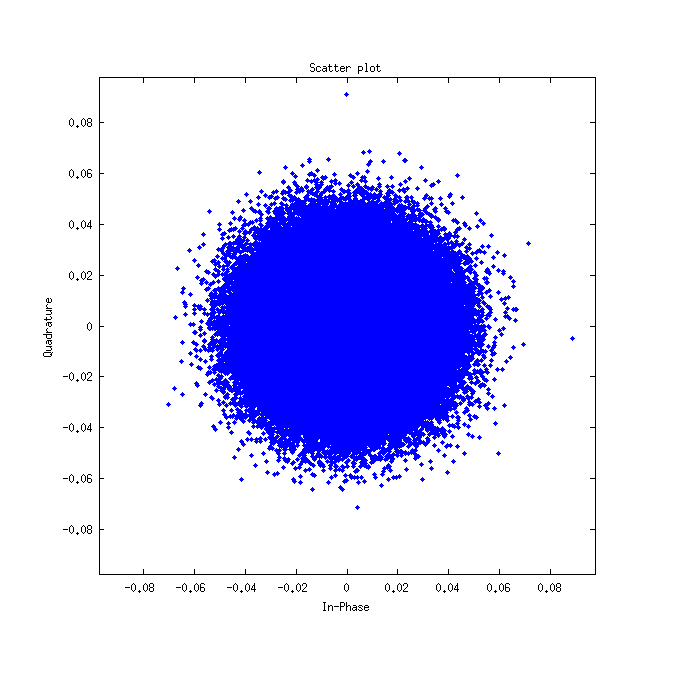
\includegraphics[width=2.2in]{4.eps}
\caption{训练中误差曲线}
\label{fig:side:a}
\end{minipage}%
\begin{minipage}[t]{0.5\linewidth}
\centering
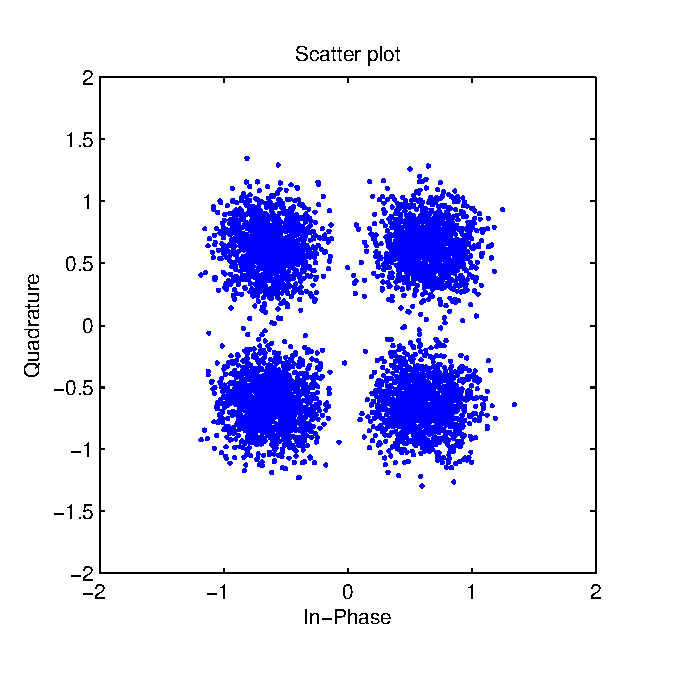
\includegraphics[width=2.2in]{5.eps}
\caption{均衡化后星座图}
\label{fig:side:b}
\end{minipage}
\end{figure}
可以看到,均衡化后,原本的四个qpsk点被恢复,效果非常明显。
\subsection*{d. BER曲线}
取信噪比 SNR=[0:15]dB,给出c)中未知序列经过均衡处理后的误码率(BER)曲线。
注意,纵坐标请用对数坐标表示。与AWGN信道下QPSK调制的标准BER曲线对比。\\
代码在main2.m,使用一个简单的平坦分部噪音来模拟噪声。效果图如下:
和AWGN信道下BER曲线对比,我采用的平坦噪声变化接收端星座图更加混乱,误码率也会更加高。
\begin{figure}[h]
\begin{minipage}[t]{0.32\linewidth}
\centering
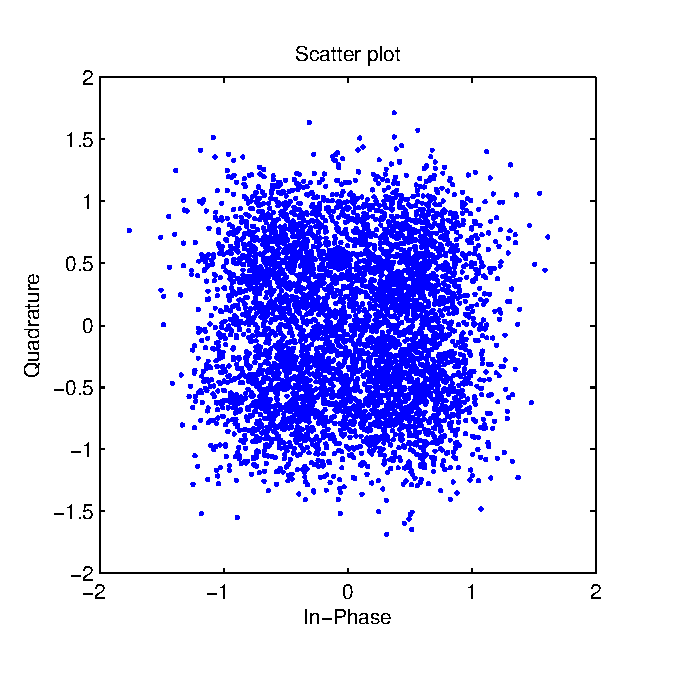
\includegraphics[width=1.2in]{61.eps}
\end{minipage}%
\begin{minipage}[t]{0.32\linewidth}
\centering
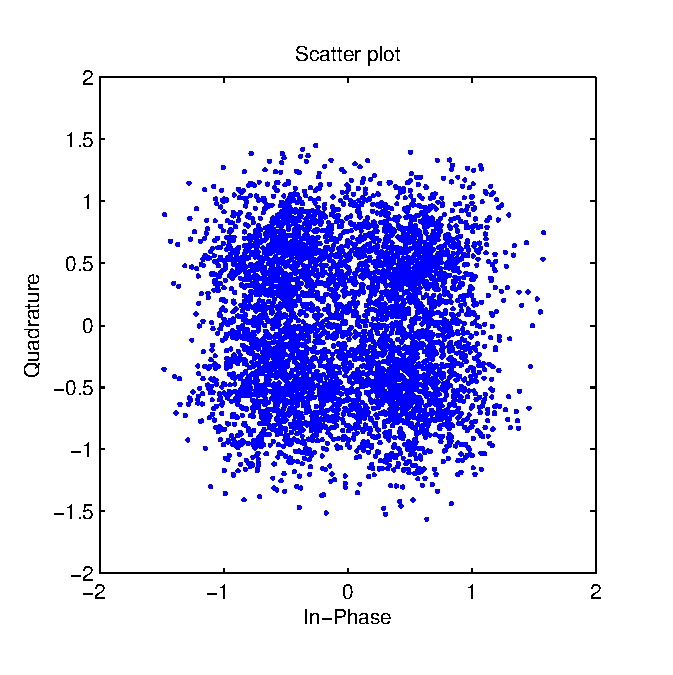
\includegraphics[width=1.2in]{62.eps}
\end{minipage}%
\begin{minipage}[t]{0.32\linewidth}
\centering
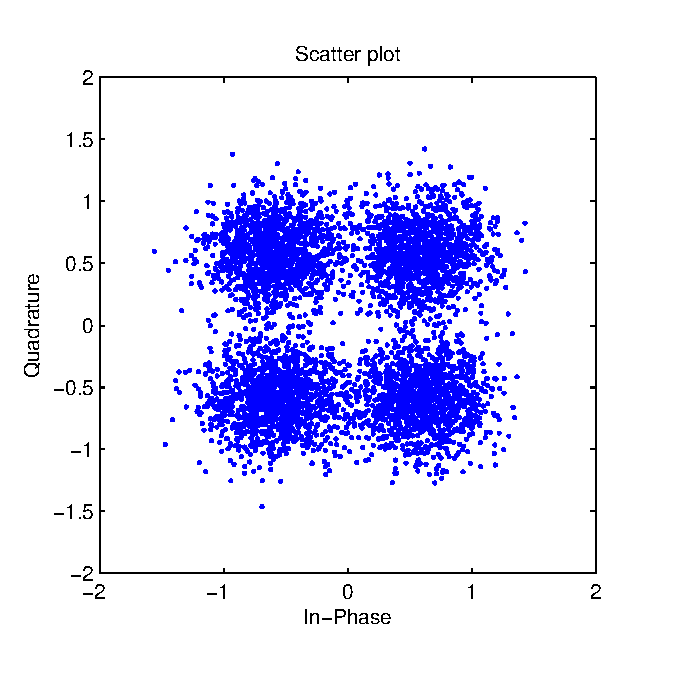
\includegraphics[width=1.2in]{65.eps}
\end{minipage}%
\end{figure}
\begin{figure}[h]
\begin{minipage}[t]{0.32\linewidth}
\centering
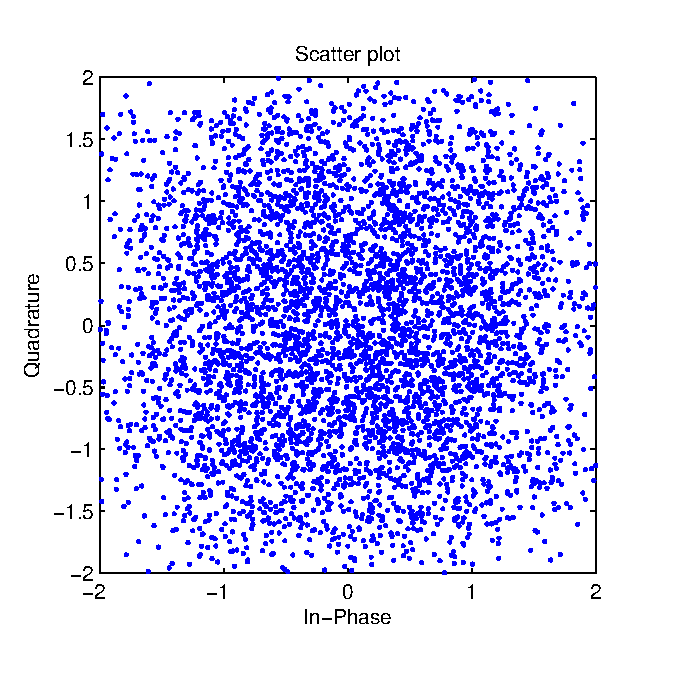
\includegraphics[width=1.2in]{71.eps}
\end{minipage}%
\begin{minipage}[t]{0.32\linewidth}
\centering
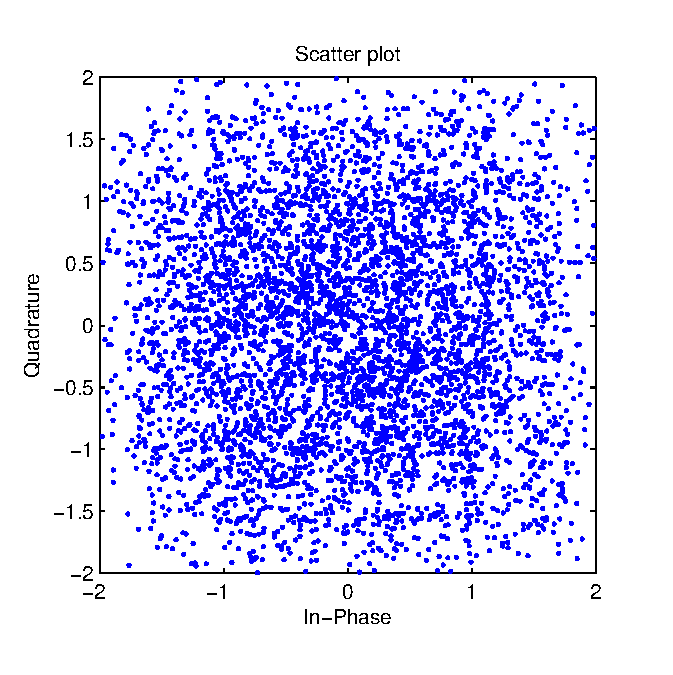
\includegraphics[width=1.2in]{72.eps}
\end{minipage}%
\begin{minipage}[t]{0.32\linewidth}
\centering
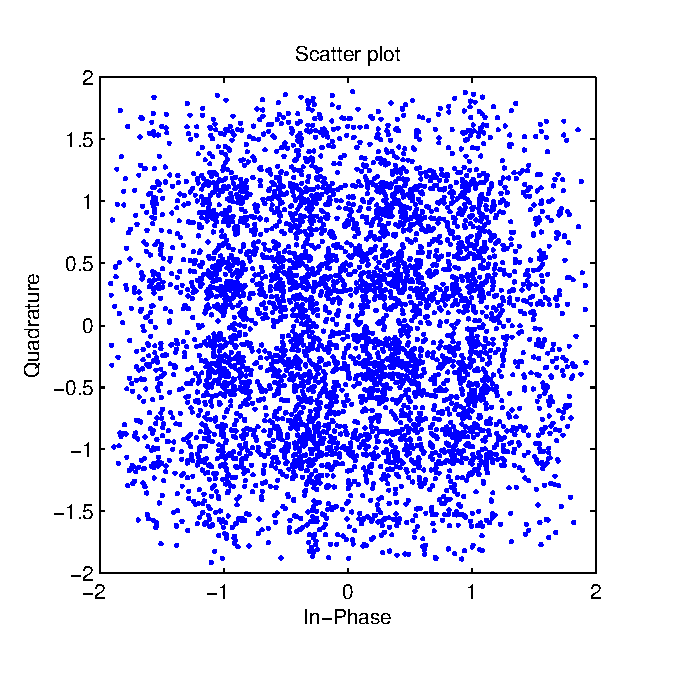
\includegraphics[width=1.2in]{75.eps}
\end{minipage}%
\end{figure}
\begin{figure}[h!]
\centering
\includegraphics[width=9cm]{8.eps}
\caption{BER误差曲线}
\end{figure}
\subsection*{e. Blind LMS}
 (选做)在某些特定场景下,我们无法知道训练序列,或者为了提高传输效率而不
采用训练序列。此时可以采用盲均衡技术对接收信号进行处理。请调研一种针对
QPSK的盲均衡算法,并重复c)和d)中的仿真。\\
这里采用一个简单的oversample的方法来解决Blind LMS的问题。
我们使用的论文是[1]中的方法。通过过采样,我们将每一个数据发送多个copy。对数据进行交织编码,打乱顺序,从而减少信道影响。\\
\noindent [1] {Watanabe, K. and Komatsu, M. and Matsumoto, H. and Furukawa, T.}, 2013.\ \lq \lq A proposal of blind equalization algorithm using over-sampling for received signals including noise. \rq \rq\ \emph{Intelligent Signal Processing and Communications Systems (ISPACS), 2013 International Symposium on}\\
可以从图7中看到,这个算法是非常有效的。不过代价是传输了重复的信息来增加准确度。
\begin{figure}[t!]
\centering
\includegraphics[width=9cm]{9.eps}
\caption{该算法BER曲线}
\end{figure}
\section{作业二}
当测量小尺度传播时,假设连续采样值在时间上有很强的相关性,需要确定合适的空间采样间隔。
假设某信号的载频为f=2700MHz,移动速率为v=35m/s,求该信号的多普勒频移\(f_m\)是多少?
再假设能够在运动的车辆上实时地进行测量,请问移动20m需要多少采样值?
(若相干时间定义为相干函数大于0.5时的时间,则相干时间可近似为:\(T_C = 9/(16\pi f_m)\))\\
\begin{equation}
	f_m = \frac{v}{\lambda} = \frac{vf}{c} = 315\mbox{Hz}
\end{equation}
想干时间计算得:
\begin{equation}
T_c = \frac{9}{16\pi f_m} = 0.000568s
\end{equation}
因此只要采样时间间隔大于相干时间
\begin{equation}
n = \frac{20\mbox{m}}{vT_c} = 1005.3
\end{equation}
最多采样100个,超出的话会发生信号堆叠。
\section{作业三}
OFDM系统的参数设计。
假设系统要求的总业务速率为R=100Mbps,
可以容忍的时延扩展为\(\tau\)=50ns,
系统信号带宽W=80MHz,请设计满足要求的OFDM系统基本参数,
包括OFDM符号周期、保护间隔、子载波数目及调制方式和纠错编码码率。\\
时延来自于并串转换时的等待时间。
假设时延是\(\tau = 39\mbox{ns}\),我们设保护时间为1ns。
于是这个时候一路信号的带宽为:
\begin{equation}
\Delta f = 1 / 38 = 26.315 \mbox{MHz}
\end{equation}
于是这个时候我们可以得到4路子载波。
这个时候的业务速率为:
\begin{equation}
R = \frac{4}{39} = 102.5\mbox{Mbps}
\end{equation}
调制方式就是最简单的IFFT+FFT调制解调方式,每102.5M个symbol我们取出其中的2.5M均匀分配作为循环校验码来进行纠错。
\section{作业四}
列举三个全球第三代移动通信系统标准,各采用何种双工方式和多址方式?
请分别谈谈你对于“双工”和“多址”的理解。\\
常见的集中第三代移动通信系统标准中,WCDMA使用的是FDD-TDD同时存在的DS-CMDA多址方式。
CDMA2000使用的是FDD,DS-CDMA,MC-CDMA多址方式。
TD-SCDMA使用的是TDD的TD-SCDMA多址方式。\\
对于多址技术,当多个用户通过基站通信,基站必须能够对用户进行识别区分。这样就可以保证基站同时和多个用户进行可靠的服务。
双工技术则是,当基站和用户进行通信时,既可以上行传输,也可以下行传输。常采用的技术有时分双工(TDD)和频分双工(FDD)。
\section{作业五}
移动通信系统中,小区(蜂窝)正在朝着越来越小的方向演化,试分析蜂窝变小可能带来的好处和问题。\\
蜂窝变小的好处有:用户容量大,服务性能较好,频谱利用率高。
带来的问题有:系统网络复杂,规划问题复杂,cell间干扰变大。
\section{作业六}
请简述ad-hoc网络中节能的主要技术。为何节能对于ad-hoc网络具有重要的意义?
Ad Hoc网络主要应用于不能提供固定设施的场合。由于有限的电池寿命,能量是非常珍稀的资源。
在网络层可以使用以下技术:最小能量路由,网络负荷平衡,休眠机制。
在数据链路层有:合理休眠,高效重传,合理设计协议以避免冲突。在物理层有:功率控制包括拓扑控制,最小能量路由,自适应功率控制
\section{作业七}
目前认知无线电的发展主要存在哪些问题?\\
从硬件的角度来说,我们可以看到:可重配置硬件平台的功能需要逐步完善;
从频谱的角度来说:频谱管制政策;
从算法的角度来说:频谱检测算法的可靠性可以提高;
算法的资源利用率需要提高;
组网协议需要完善。
\section{作业八}
超宽带(UWB)系统的三种主要体制是什么?具有哪些特点?存在哪些不足?\\
脉冲超宽带技术(IR-UWB)目前仍然在理论阶段,物理层设计与传统系统有很大差异。极窄脉冲波形,占空比低。
直接序列超宽带技术(DS-UWB),可以将频谱分成2个子带。子带采用三电平高速直扩方法,使用QPSK/BPSK调制。
技术和以往的技术差别较小,效果有限。\\
多带正交频分复用超宽带技术(MB-OFDM-UWB),将可用频谱分成13个子带,每个子带宽度528MHz,128个正交载波,QPSK调制。
MB-OFDM-UWB系统与其他系统之间的电磁兼容问题较差,因此其发射功率受到严格的限制。
\section{作业九}
列举两个典型的商用卫星移动通信系统。它们均采用什么轨道高度的卫星?不采用GEO卫星系统的原因有哪些?\\
铱系统的轨道高度为780公里,而全球星系统的轨道高度为1414公里。
两者不采用GEO卫星系统的共同原因是外太空信号衰减大,信号延时长,轨道资源紧张。
\section{作业十}
试分析地面无线移动通信与卫星通信中所采用的信道模型有何不同?请举例说明?\\
地面无线通信中采用多径信道。这是因为地面信号传输过程中存在非常普遍的障碍物反射,衍射,散射影响。移动物体的运动速度和方向引起的多普勒效应也会造成影响。
而在卫星通信中,延时大,突发错误率高,
损耗主要来自于大气损耗,大气折射损耗,天线跟踪误差损耗,极化误差损耗等。同时要考虑的噪声包括热噪声,太阳噪声,大气噪声,降雨噪声,地面噪声,互调噪声。
因此两者模型不同。
\end{CJK}
\end{document}